\problem{Color space conversion}

1. Convert RGB image to HSI image.\\
The formula to convert RGB to HSI is as follows:
\begin{align*}
    \theta &= \arccos\left\{ \dfrac{\frac{1}{2} [(R-G)+(R-B)]}{\left[(R-G)^2+(R-B)(G-B)\right]^{\frac{1}{2}}} \right\} \\
    H &= \begin{cases}
        \theta & \text{if } B \leq G \\
        360 - \theta & \text{if } B > G
    \end{cases} \\
    S &= 1 - \dfrac{3}{R+G+B} \min\{R,G,B\} \\
    I &= \dfrac{R+G+B}{3}
\end{align*}
And the HSI channels should be normalized to $[0,1]$.\\
Since $H$ represents the hue, which is a circular value, and its range is $[0,360]$.\\
$S$ represents the saturation, its range is $[0,1]$.\\
$I$ represents the intensity, its range is $[0,255]$.\\
So to normalize the HSI channels, we can use the following formula:
$$H \gets \dfrac{H}{360}, S \gets \dfrac{S}{1}, I \gets \dfrac{I}{255}$$
For details, since we need to avoid the situation that the denominator is $0$, so we can add $\epsilon = 10^{-9}$ on
the denominator when calulating $\theta$ and $S$.\\
Also, in order to fit the domain of the function $\arccos$, we need to clip the values into $[-1,1]$ when calulating $\theta$.\\
So with above formulas, we can convert the RGB image to HSI image.\\

2. Convert HSI image to RGB image.\\
The formula to convert HSI to RGB is as follows:
\begin{align*}
    & 0^{\circ} \leq H<120^{\circ} \\
    & B=I(1-S), \quad R=I\left[1+\frac{S \cos (H)}{\cos \left(60^{\circ}-H\right)}\right], \quad G=3 I-(R+B) \\
    & >120^{\circ} \leq H<240^{\circ} \\
    & R=I(1-S), \quad G=I\left[1+\frac{S \cos \left(H-120^{\circ}\right)}{\cos \left(180^{\circ}-H\right)}\right], \quad B=3 I-(R+G) \\
    & >240^{\circ} \leq H<360^{\circ} \quad \\
    & G=I(1-S), \quad B=I\left[1+\frac{S \cos \left(H-240^{\circ}\right)}{\cos \left(300^{\circ}-H\right)}\right], \quad R=3 I-(G+B)
\end{align*}

And the RGB channels should be normalized to $[0,255]$.\\
So to normalize the RGB channels, we need to recover the HSI by using the following formula:
$$H \gets H*360, S \gets S*1, I \gets I * 255$$
For specific details, all values of $H$ are using the radians, so the numbers of the degrees above should be converted to radians while implementing.\\
With these formulas, we can convert the HSI image to RGB image.\\
With the analysis above, we can convert the RGB image to HSI image, and recover the RGB image from the HSI image.\\
The Figure \ref{fig:p3} is the result of the conversions.\\

\begin{figure}[htbp]
    \centering
	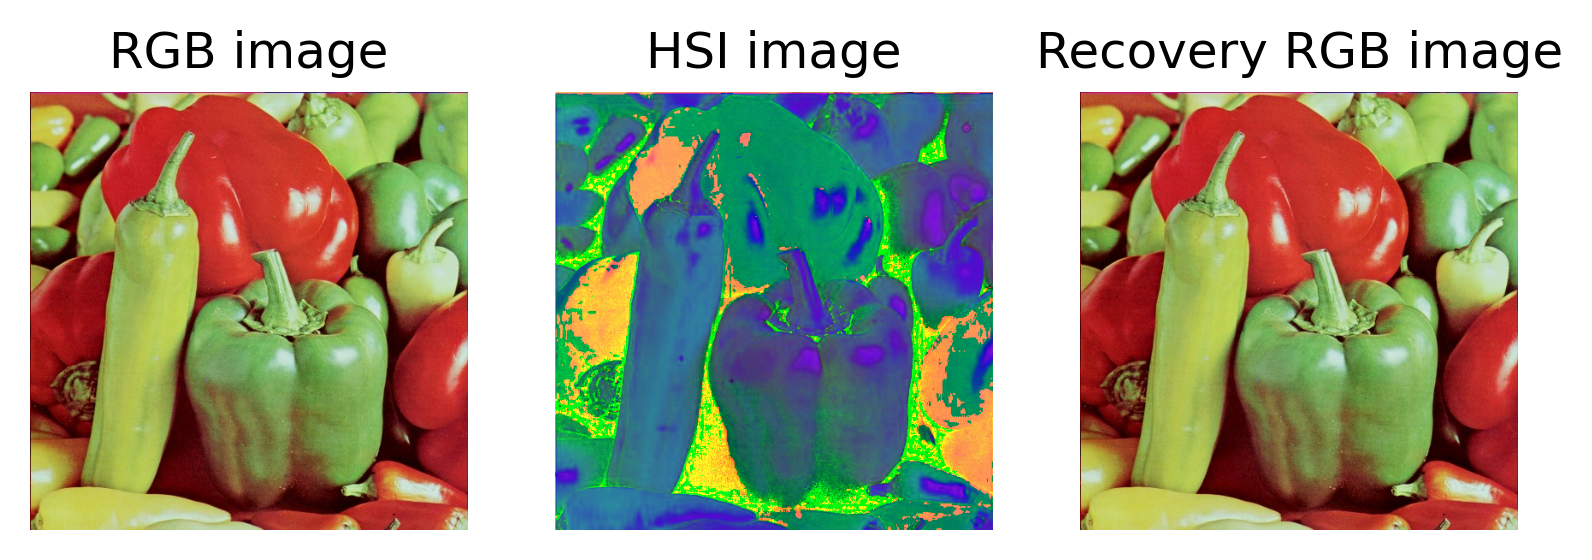
\includegraphics[width=\textwidth]{../images/p3/p3.png}
    \caption{RGB to HSI conversion and the recovery}
    \label{fig:p3}
\end{figure}
\newpage